% siminos/atlas/flotsam.tex    master file: main.tex
% $Author$ $Date$

\section{Flotsam}
\label{s:flotsam}

\noindent
{\bf [2012-03-12 Predrag]}
\\
How to use this section? When you remove cogent text from the article
proper - clip  it and paste it into here, for possible reuse later.

\subsection{Introduction}
\label{s:introFlot}

Making full use of these ideas necessitates reexamination of two of the
basic tools of the theory of dynamical systems, Poincar\'e sections and
symmetry reduction.

    in order to motivate the need for continuous symmetry reduction , explain
    what it is, and how with it the geometry of \statesp\ dynamics is revealed;


The importance of a given invariant solution is made precise by periodic
orbit theory which assigns a deterministic weight with which the solution
contributes to any dynamical average over the chaotic component of the
flow \rf{DasBuch}. Consideration of continuous symmetries extends this
theory to sums over \emph{relative} periodic orbits\rf{Cvi07},
time-dependent solutions which recur periodically in co-moving frames
translating along and/or rotating about the axes of symmetry with
different translational and rotational velocities for each solution.

The $\infty$-dimensional \stateDsp\
representation\rf{GHCW07} of PDEs, such as \reffig{f:MeanVelocityFrame},
enables us to track the unstable manifolds of invariant
solutions, the heteroclinic connections between them\rf{GHCV08}, and
{provides us with} new insights into the nonlinear \statesp\ geometry and
dynamics of moderate \Reynolds\ wall-bounded flows.

%%%%%%%%%%%%%%%%%%%%%%%%%%%%%%%%%%%%%%%%%%%%%%%%%
% 2011-10-23 Predrag: replace this Ashley' simulation
%            continuous.tex overheads, and ChaosBook
% TEMPORARY: from siminos/rpo_ks/arxiv-v2/figs, \refref{cont:SCD07})
%
\begin{figure}
\centering
(a)%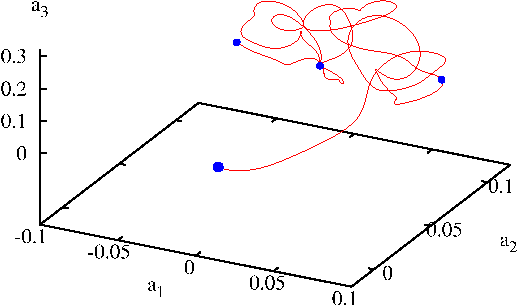
\includegraphics[width=0.45\textwidth,clip=true]{2841GO3a}
~~(b)%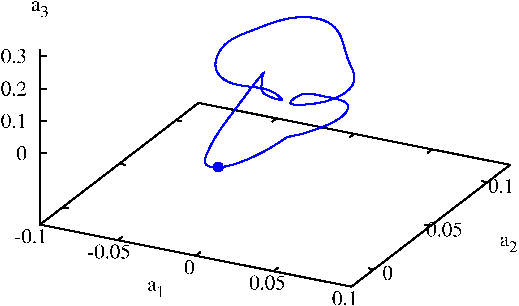
\includegraphics[width=0.45\textwidth,clip=true]{2841GO3b}
  \caption{\label{f:MeanVelocityFrame}
Symmetry reduction $\pS \to \pSRed$ replaces each
(a)
full \statesp\ trajectory $\ssp(\zeit)$ by
(b)
a simpler \reducedsp\ trajectory $\sspRed(\zeit)$, with continuous group
induced drifts quotiented out. Here this is illustrated by the pipe flow \rpo\
$\RPO{36.92}$
(a) %(red)
traced in the full {\statesp} for two $\period{}=36.92$ periods, in the
frame moving with the constant mean axial flow speed $U$;
(b) %(blue)
restricted to the symmetry-\reducedsp. Both are projected onto the
$3$\dmn\ frame \refeq{FrenetFrame1}. In the full \statesp\ a \rpo\ traces
out quasi-periodically a highly contorted 2-torus; in the \reducedsp\ it
closes a \po\ in one period $\period{}$.
            }
\end{figure}
%%%%%%%%%%%%%%%%%%%%%%%%%%%%%%%%%%%%%%%%%%%%%%%%%%

We review  ??? flows, their visualization, and their symmetries in
\refsect{s:review}. The {\mslices}  is described in \refsect{s:slice},
and the computation of invariant solutions and their stability
eigenvalues and eigenvectors in \refsects {sect:TimeOrb}{s:algorithm}.
The main advances reported in this paper are the symmetry \reducedsp\
visualization and [...], (\refsect{s:rpos}). Outstanding challenges are
discussed in \refsect{s:concl}.

% \subsection{Pipe flows}
% \label{s:reviewFlot}
% former siminos/atlas/review.tex    master file: main.tex

As long as one is focusing on a single solution of \NSe, there are many
excellent, physically insightful $3D$ visualizations of the flow:
velocity fields on flow sections, isovorticity surfaces, videos of the
flow, and so on. But today we own dozens of exact \eqv\ and \reqv\
solutions for a given turbulent flow, and we are commencing an exploration of
states of turbulent fluids in terms of the unstable \po\ solutions whose
number, as a function of the increasing period, is growing exponentially.
How are we to visualize \emph{the totality} of these solutions in one go?

The answer was given by \cite{hopf48}, who envisioned the function space
of {\NS} velocity fields as an infinite-dimensional \statesp\ $\pS$ in
which each instantaneous state of $3D$ fluid velocity field $\vec{u}(\bx)$ is
represented as a unique point $\ssp$. In our particular application we
can represent $\ssp = (\vec{u}_{nkm})$ as a vector whose elements are the
primitive discretization variables \refeq{pipeDiscr}. The $3D$ velocity
field given by $\vec{u}_{knm}(\zeit)$, obtained from integration of the
\NSe\ in time, can hence be seen as trajectory $\ssp(\zeit)$ in
$\approx 100,000$ dimensional space spanned by the free variables of our
numerical discretization, with the \NS\ equations \refeq{NavStokesDev}
rewritten as
\beq
   \dot{\ssp} = \vel(\ssp) ,
   \qquad
   \ssp(\zeit) = \ssp(0)
            + \int_0^\zeit \! \mathrm{d}\zeit' \, \vel(\ssp(\zeit'))
\,,
\ee{symbolicNS}
where the current state of the fluid $ \ssp(\zeit)$ is the time-$\zeit$
forward map of the initial fluid state  $\ssp(0)$.

On perils of thinking linearly: bases such as Fourier modes are
perfectly natural for problems such a bifurcation of a steady state, and
other weak perturbations. They are absolutely unnatural for strongly
nonlinear problems, with many Fourier modes of comparable magnitude and
strongly entangled.

        There is always tension between mathematics - linear problem eigenmodes
        (Fourier for translations and rotations) and physics - the fact that
        nonlinear dynamics states are far away from such axes, as they
        always involve a number of such linear modes strongly entangled.

In order to quantify whether two fluid states are close to or far from
each other, one needs a notion of distance between two points in
\statesp, measured here as
\beq
  \Norm{\ssp-\ssp'}^2  = \braket{\ssp-\ssp'}{\ssp-\ssp'} =
\frac{1}{V}
\int_\bCell \! d \bx \;
(\vec{u}-\vec{u}') \cdot (\vec{u}-\vec{u}')
\,.
\ee{innerproduct}
There is no compelling reason to use this {`energy norm'}, other than
that velocity fields is what is given in a numerical computation. What
norm one actually uses depends very much on the application.
Visualizations of trajectory \refeq{symbolicNS} are of necessity
projections onto two or three dimensions.

Recently, \cite{GHCW07} have shown that the dynamics of different regions
of {\statesp}, considered as a high-dimensional vector space, can be
elucidated more profitably by a computationally straight\-forward sets of
\emph{physical} coordinates. One identifies several prominent states of
the flow $\vec{u}_A$, $\vec{u}_B$, $\dots$, such as {\eqv} states and
their linearized stability eigenvectors, states in whose neighborhoods
the turbulent flow spends most of the time, and from them constructs, by
Gram-Schmidt or (anti)-symmetrizations, an orthonormal basis set
$\{\be_1, \be_2, \cdots, \be_n\}$. The evolving fluid state $\bu(\zeit)$
is then projected onto this basis using the inner product
\refeq{innerproduct},
\beq
\ssp(\zeit) =(\ssp_1, \ssp_2, \cdots, \ssp_n, \cdots)(\zeit)
    \,,\qquad
\ssp_n(\zeit) = \braket{\vec{u}(\zeit)}{\be_n}
\,.
\ee{intrSspTraj}
Low-dimensional projections of the flow can be viewed in any of the $2D$ planes
$(\ssp_m, \ssp_n)$ or in $3D$ perspective views $(\ssp_{\ell},\ssp_m,
\ssp_n)$. An example is the \reffig{f:MeanVelocityFrame} projection on
the $3$\dmn\ frame $\{{\be}_1,{\be}_2,{\be}_3\}$ defined in \refeq{FrenetFrame1}.
It is worth emphasizing that the method affords low-dimensional {\em
visualization} without any low-dimensional {\em modeling} or dimension
reduction; the dynamics are computed with fully-resolved direct numerical
simulations.

Such visualizations are a prerequisite to uncovering the
interrelations between (the infinite number of) invariant solutions, and
constructing symbolic dynamics partitions of \statesp\ needed for a
systematic exploration of turbulent dynamics, the key challenge that we
address here for the case of turbulent pipe flows.

\subsection{Experimentalist description: a video 1D to 3D arrays of pixels}
\subsection{Theorist description: $\infty$-\dmn\ \statesp}

\subsubsection{Poincar\'e sections}
\label{s:PoincSecFlot}

%%%%%%%%%%%%%%%%%%%%%%%%%%%%%%%%%%%%%%%%%%%%%%%%%%%%%%%%%%%%%%%%%%%%%
\begin{figure}
   \centering
(a)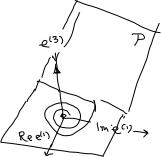
\includegraphics[width=0.20\textwidth]{A29PoincBad}
(b)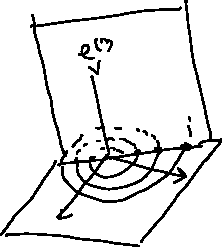
\includegraphics[width=0.20\textwidth]{A29PoincGood}
   \caption{\label{fig:A29PoincBad}
A Poincar\'e section should capture important features of the local flow.
    (a)
A section through a \template\ off the invariant set is bad, as it misses
dynamics around a nearby \eqv.
    (b)
If an \eqv\ is chosen as a \template, the section is good - it captures
all local dynamics.
}
\end{figure}
%%%%%%%%%%%%%%%%%%%%%%%%%%%%%%%%%%%%%%%%%%%%%%%%%%%%%%%%%%%%%%%%%%%%%

%%%%%%%%%%%%%%%%%%%%%%%%%%%%%%%%%%%%%%%%%%%%%%%%%%%%%%%%%%%%%%%%%%%%%
\begin{figure}
   \centering
   %\includegraphics[width=0.45
\begin{minipage}[b]{0.19\textwidth} %{0.39\textwidth}
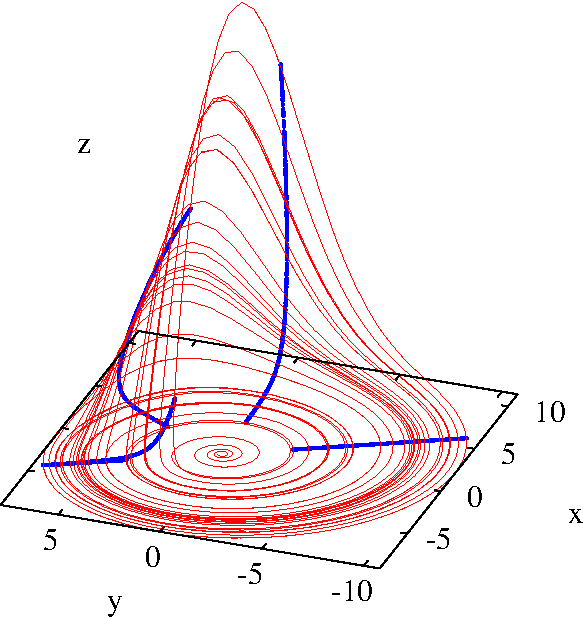
\includegraphics[width=1.15\textwidth,origin=c]
            {Rossler_PsectionB}
\\
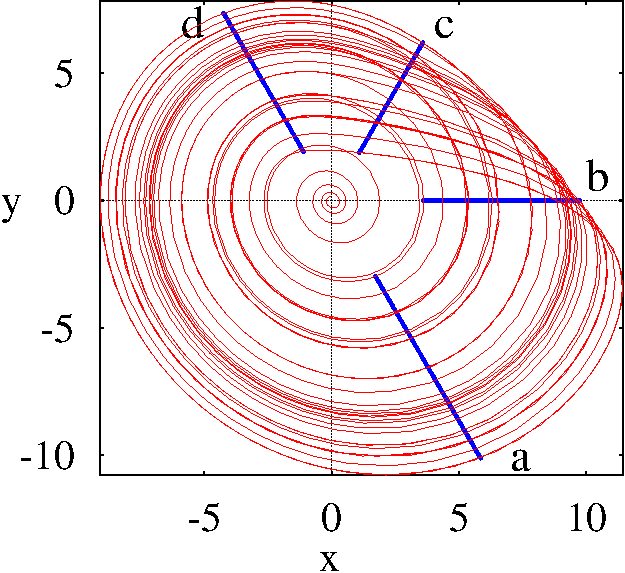
\includegraphics[width=0.80\textwidth,origin=c]
            {Rossler_PsectionA}
  \end{minipage}~~~~~%
  \begin{minipage}[b]{0.25\textwidth} %{0.50\textwidth}
    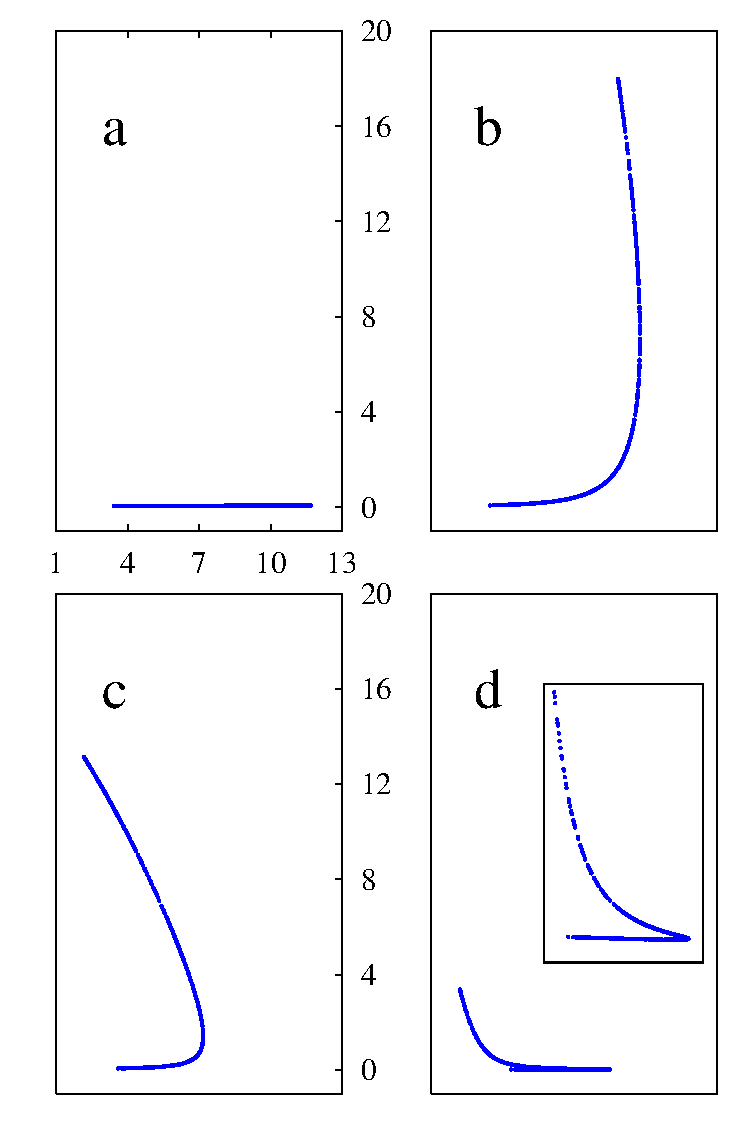
\includegraphics[width=1.00\textwidth]
            {Rossler_PsectionC}
  \end{minipage}
   \caption{\label{f:RosslSect}
      (Right) a sequence of Poincar\'e sections of
      the R\"ossler strange attractor,
      defined by planes through the $z$~axis, oriented at angles
      (a) $-60^o$
      (b) $0^o$,
      (c) $60^o$,
      (d) $120^o$,
      in the $x$-$y$~plane.
      (Left) side and $x$-$y$~plane view of a typical trajectory  with
      Poincar\'e sections superimposed.
      (R. Pa\v skauskas)
            }
\end{figure}
%%%%%%%%%%%%%%%%%%%%%%%%%%%%%%%%%%%%%%%%%%%%%%%%%%%%%%%%%%%%%%%%%%%%%

%%%%%%%%%%%%%%%%%%%%%%%%%%%%%%%%%%%%%%%%%%%%%%%%%%%%%%%%%%%%%%%%%%%%%
\begin{figure}
  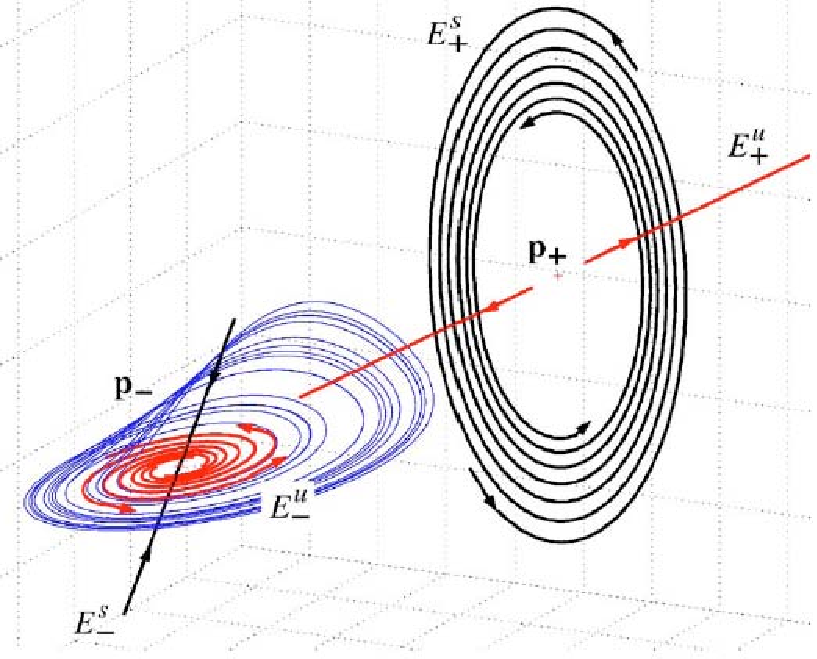
\includegraphics[width=0.3\textwidth]{AmLeAg06Im1}
    \caption{[From \refref{AmLeAg06}]
R\"ossler \eqva\ and their invariant manifolds. The stable manifold of
the inner {\eqv} $\ssp_{-}$  is 1-dimensional and the unstable one is a
spiral-out focus. For the outer {\eqv} $\ssp_{+}$  the stable manifold is
a spiral-in focus (basin boundary for initial conditions that either fall
into the chaotic attractor, or escape to infinity) and the unstable
manifold is 1-dimensional.
    }
\label{fig:AmLeAg06Im1}
\end{figure}
%%%%%%%%%%%%%%%%%%%%%%%%%%%%%%%%%%%%%%%%%%%%%%%%%%%%%%%%%%%%%%%%%%%%%


%%%%%%%%%%%%%%%%%%%%%%%%%%%%%%%%%%%%%%%%%%%%%%%%%%%%%%%%%%%%%%%%%%%%%
\begin{figure}%[H]
\begin{center}
  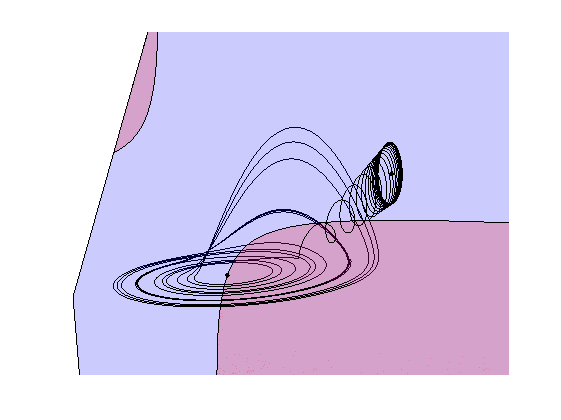
\includegraphics[width=0.30\textwidth,clip=true]{RoessNearEq}
\end{center}
  \caption{\label{fig:RoessNearEq1}
  A R\"ossler flow Poincar\'e section $\PoincS_{-}$ through the inner
  {\eqv} $\ssp_{-}$ and its stable eigenvector.
}
\end{figure}
%%%%%%%%%%%%%%%%%%%%%%%%%%%%%%%%%%%%%%%%%%%%%%%%%%%%%%%%%%%%%%%%%%%%%

%%%%%%%%%%%%%%%%%%%%%%%%%%%%%%%%%%%%%%%%%%%%%%%%%%%%%%%%%%%%%%%%%%%%%
\begin{figure}%[H]
\begin{center}
  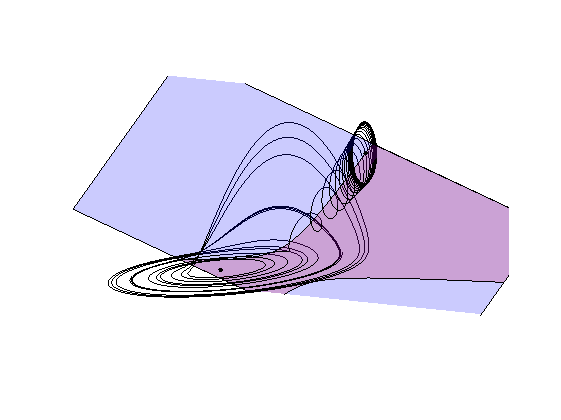
\includegraphics[width=0.30\textwidth,clip=true]{RoessFarEq}
\end{center}
  \caption[R\"ossler section, outer {\eqv}]{
  A Poincar\'e section for R\"ossler flow
      through the
      outer
  {\eqv} $\ssp_{+}$  and its unstable eigenvector.
  } \label{fig:RoessFarEq1}
\end{figure}
%%%%%%%%%%%%%%%%%%%%%%%%%%%%%%%%%%%%%%%%%%%%%%%%%%%%%%%%%%%%%%%%%%%%%

%%%%%%%%%%%%%%%%%%%%%%%%%%%%%%%%%%%%%%%%%%%%%%%%%%%%%%%%%%%%%%%%%%%%%
\begin{figure}%[H]
\begin{center}
  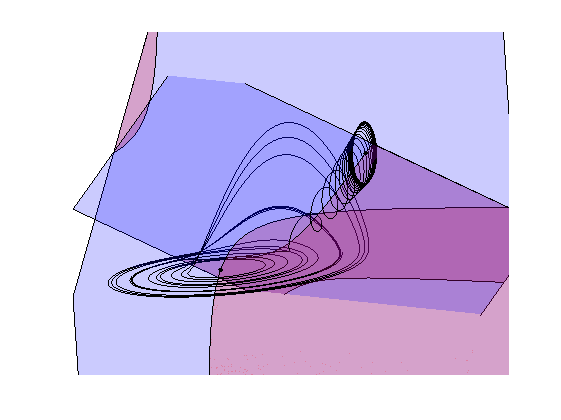
\includegraphics[width=0.30\textwidth,clip=true]{RoessBothEq}
\end{center}
  \caption{
  A two-section atlas for R\"ossler flow, with the local sections of
  \reffigs{fig:RoessNearEq}{fig:RoessFarEq} oriented and combined so that
  the ridge (intersection of the two sections, indicated by the brown
  line in individual sections) lies  approximately midway between the
  \template s.
  } \label{fig:RoessBothEq1}
\end{figure}
%%%%%%%%%%%%%%%%%%%%%%%%%%%%%%%%%%%%%%%%%%%%%%%%%%%%%%%%%%%%%%%%%%%%%

%%%%%%%%%%%%%%%%%%%%%%%%%%%%%%%%%%%%%%%%%%%%%%%%%%%%%%%%%%%%%%%%%%%%%
\begin{figure}%[H]
\begin{center}
  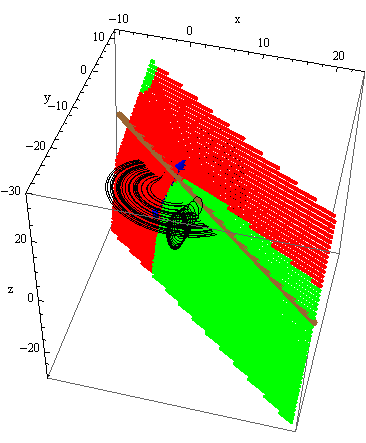
\includegraphics[width=0.30\textwidth,clip=true]{RoessSct1}
\end{center}
  \caption{\label{fig:RoessSct1}
  A R\"ossler flow Poincar\'e section $\PoincS_{-}$ through the inner
  {\eqv} $\ssp_{-}$ and its stable eigenvector.
}
\end{figure}
%%%%%%%%%%%%%%%%%%%%%%%%%%%%%%%%%%%%%%%%%%%%%%%%%%%%%%%%%%%%%%%%%%%%%

%%%%%%%%%%%%%%%%%%%%%%%%%%%%%%%%%%%%%%%%%%%%%%%%%%%%%%%%%%%%%%%%%%%%%
\begin{figure}%[H]
\begin{center}
  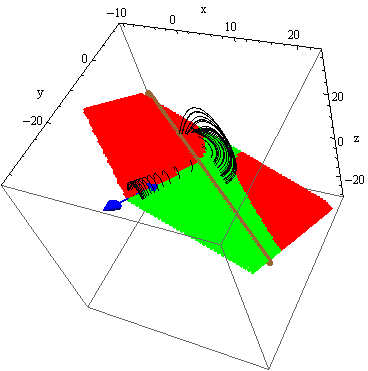
\includegraphics[width=0.30\textwidth,clip=true]{RoessSct2}
\end{center}
  \caption[R\"ossler section, outer {\eqv}]{
  A Poincar\'e section for R\"ossler flow
      through the
      outer
  {\eqv} $\ssp_{+}$  and its unstable eigenvector.
  } \label{fig:RoessSct2}
\end{figure}
%%%%%%%%%%%%%%%%%%%%%%%%%%%%%%%%%%%%%%%%%%%%%%%%%%%%%%%%%%%%%%%%%%%%%

%%%%%%%%%%%%%%%%%%%%%%%%%%%%%%%%%%%%%%%%%%%%%%%%%%%%%%%%%%%%%%%%%%%%%
\begin{figure}%[H]
\begin{center}
  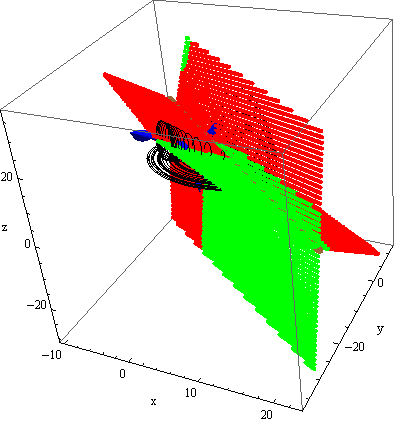
\includegraphics[width=0.30\textwidth,clip=true]{RoessSctAtlas}
\end{center}
  \caption{
  A two-section atlas for R\"ossler flow, with the local sections of
  \reffigs{fig:RoessSct1}{fig:RoessSct2} oriented and combined so that the ridge (intersection
  of the two sections, indicated by the brown line in individual
  sections) lies  approximately midway between the \template s.
  } \label{fig:RoessSctAtlas}
\end{figure}
%%%%%%%%%%%%%%%%%%%%%%%%%%%%%%%%%%%%%%%%%%%%%%%%%%%%%%%%%%%%%%%%%%%%%

 A
section that passes through either of these points captures nearby
trajectories whose short-time dynamics resembles that of the \template.

 As their local
dynamics is nonlinear and qualitatively different, no single section can
describe the neighborhoods of the both templates well.

A section through a \template\ off the invariant set is bad, as it misses
dynamics around a nearby \eqv.

If an \eqv\ is chosen as a \template, the section is good - it captures
all local dynamics.

\refFig{fig:A29PoincBad}\,({\it a}) shows why \reffig{f:RosslSect} is OK for
capturing the strange attractor, but actually bad; the lower \eqv\
$\ssp_{-}$ does not lie on the $z$ axis, so a section that includes the
$z$ axis misses the motions close to  $\ssp_{-}$.
%    \DB{2012-04-10}{
%    As of today `chart' is undefined in the text up to this point}
      \DB{2012-04-10}{As of today \reffig{fig:A29PoincBad} about good and bad Poincare
      sections went to Flotsam. Are we going to put it back or are we
      dropping it and should ``correctly'' be dropped.
      Predrag: I think we drop it, for brevity's sake}

%%%%%%%%%%%%%%%%%%%%%%%%%%%%%%%%%%%%%%%%%%%%%%%%%%%%%%%%%%%%%%%%%%%%%
\begin{figure}
   \centering
(a)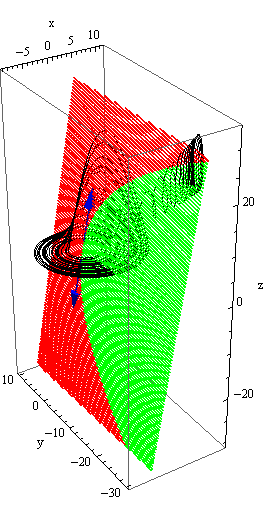
\includegraphics[width=0.16\textwidth]{robbins3-7a}
(b)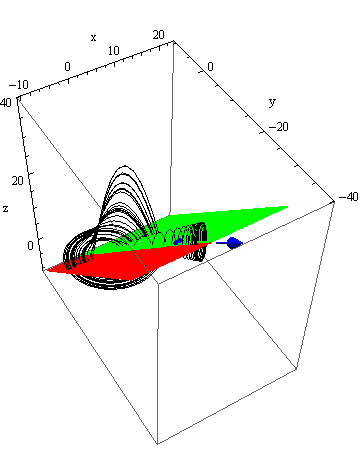
\includegraphics[width=0.24\textwidth]{robbins3-7b}
(c)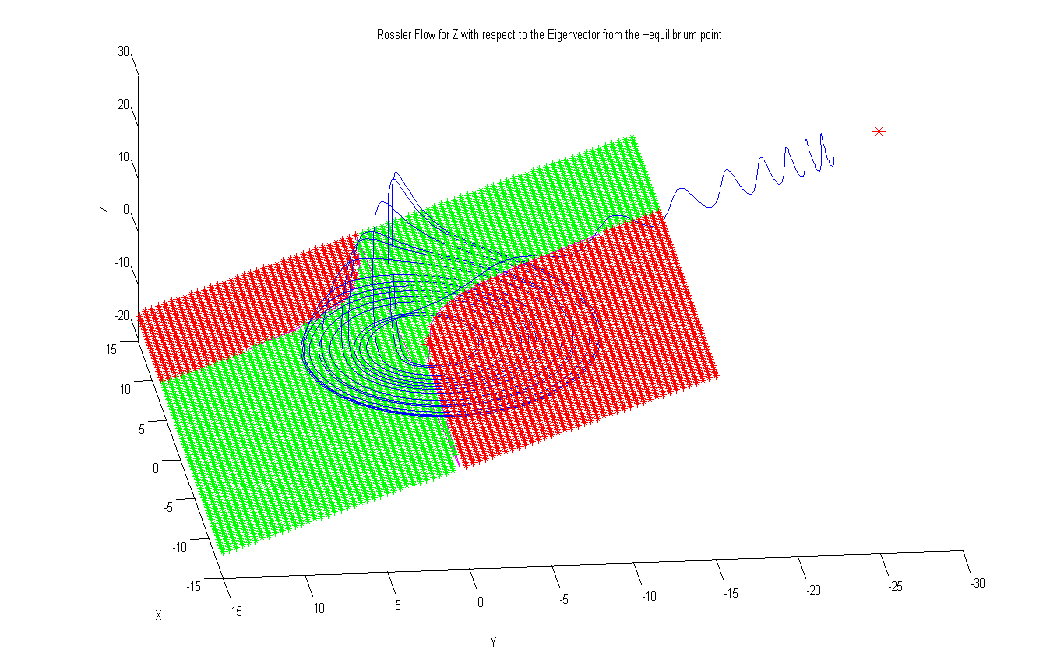
\includegraphics[width=0.44\textwidth]{wadsworth3-7a}
   \caption{\label{fig:robbins3-7}
    (a)
A section as in \refFig{fig:A29PoincBad}\,({\it b}), correctly centered
centered on $\ssp_{-}$ (Robbins).
    (b)
A section centered on $\ssp_{+}$ (Robbins).
    (c)
(Wadsworth).
}
\end{figure}
%%%%%%%%%%%%%%%%%%%%%%%%%%%%%%%%%%%%%%%%%%%%%%%%%%%%%%%%%%%%%%%%%%%%%

%%%%%%%%%%%%%%%%%%%%%%%%%%%%%%%%%%%%%%%%%%%%%%%%%%%%%%%%%%%%%%%%%%%%%
\begin{figure}
   \centering
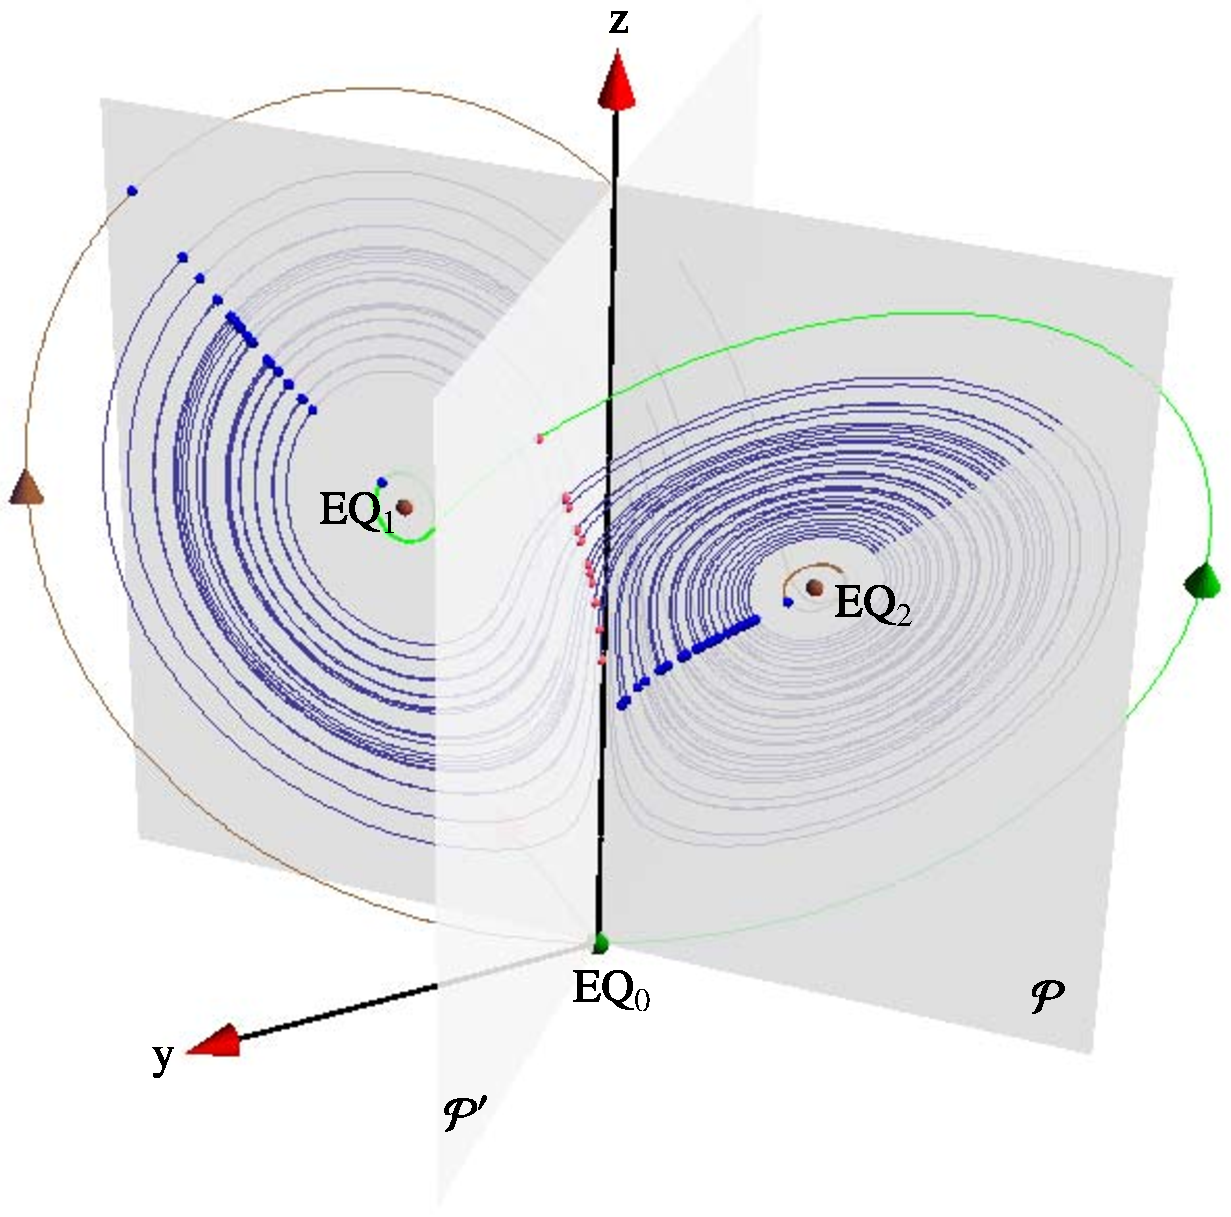
\includegraphics[width=0.40\textwidth, clip=true]{lorenz2Poinc}
   \caption{
Lorenz flow cut by  $y=x$ Poincar\'e section plane $\PoincS$ through the
$z$ axis and both $\EQV{1,2}$ \eqva. Points where flow pierces into
section % $\PoincS$ are marked by dots. To aid visualization of the flow
near the $\EQV{0}$ \eqv, the flow is cut by the second Poincar\'e
section,  $\PoincS'$, through $y=-x$ and the $z$ axis.
\hfill (from E. Siminos, ChaosBook.org)
%       \(\sigma = 10, b= 8/3, \rho = 28\,.\)
} \label{fig:LorenzSect}
\end{figure}
%%%%%%%%%%%%%%%%%%%%%%%%%%%%%%%%%%%%%%%%%%%%%%%%%%%%%%%%%%%%%%%%%%%%%


Along with continuous symmetries come important classes of invariant
solutions referred to as `relative' or `equivariant'
\rf{Huyg1673,Poinc1896}. One expects to find relative
equilibria and \rpo s\rf{Rand82}, associated with the translational
and rotational symmetries of the flow.


\subsection{R\"ossler unstable manifold curvilinear distance}

{\bf [2012-04-10 Predrag]} gave up on Keith's \reffig{fig:RoessRetMap}
and the yet undrawn {R\"ossler return map}.

%%%%%%%%%%%%%%%%%%%%%%%%%%%%%%%%%%%%%%%%%%%%%%%%%%%%%%%%%%%%%%%%%%%%%
\begin{figure}
\begin{center}
(a) % 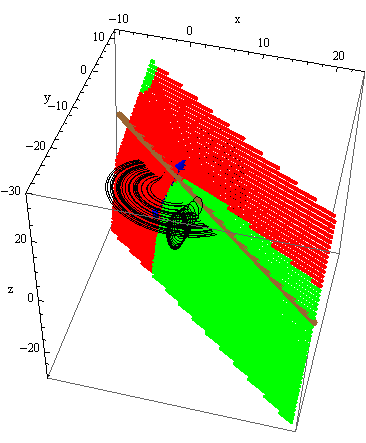
\includegraphics[width=0.30\textwidth,clip=true]{RoessSct1}
(b) 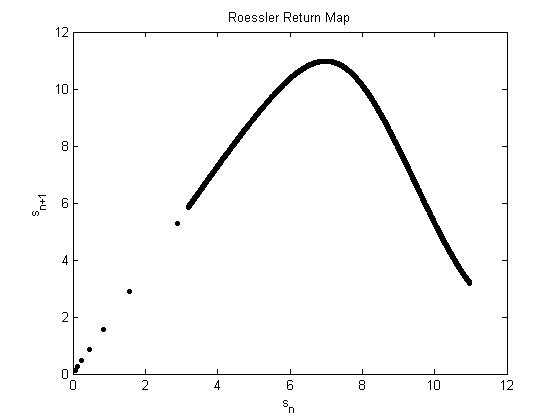
\includegraphics[width=0.30\textwidth,clip=true]{RoessRetMap}
\end{center}
  \caption{
(a) R\"ossler strange attractor section of \reffig{RoessSct1}
(b) R\"ossler return map for curvilinear distance as measured
along the unstable manifold section (the method of
\refref{Christiansen97}, see \refrefs{DasBuch,Basu07}).
  }
\label{fig:RoessRetMap}
\end{figure}
%%%%%%%%%%%%%%%%%%%%%%%%%%%%%%%%%%%%%%%%%%%%%%%%%%%%%%%%%%%%%%%%%%%%%



\subsection{Symmetries of flows}
\label{s:symmFL}

In our quest for \reqva\ and \rpo s\rf{ACHKW11} we
find it advantageous to use a `compensatory' norm %\refeq{compensNorm}
that enhances the weight of cross-stream velocities.


Any state in the  group orbit set $\pS_{\ssp}$
is physically equivalent to any other. The action of a symmetry group
thus stratifies the \statesp\ into a union of group orbits,
\reffig{fig:BeThTraj}\,{(a)}.

While in the case of \SOn{2} symmetry a \reqv\ traces out a loop in the
full \statesp (see \reffig{fig:CLf01group}, e.g.), for a
higher-dimensional continuous symmetry it explores the group orbit
$\pS_{\REQV{}{}}$ quasi-periodically, so a \reqv\ is \emph{not} a \po.
Rather, as all states in this group orbit are physically the same state
for all time, this is a generalized \eqv\ state.

Continuous symmetry parameters (`phases' or `shifts')
$\{\gSpace_j\}=\{\phi_p,\shift_p\}$ are real numbers, ratios
$\pi/\gSpace_j$ are almost never rational, and \rpo s are almost never
eventually periodic; the time evolution of a relative periodic point thus
sweeps out quasi-periodically the $3$\dmn\ group orbit $\pS_p$ without
ever closing into a \po, unless the dynamics is restricted to a
discrete-symmetry invariant subspace (\reffig{fig:CLf01group}).

\begin{figure}
\begin{center}
  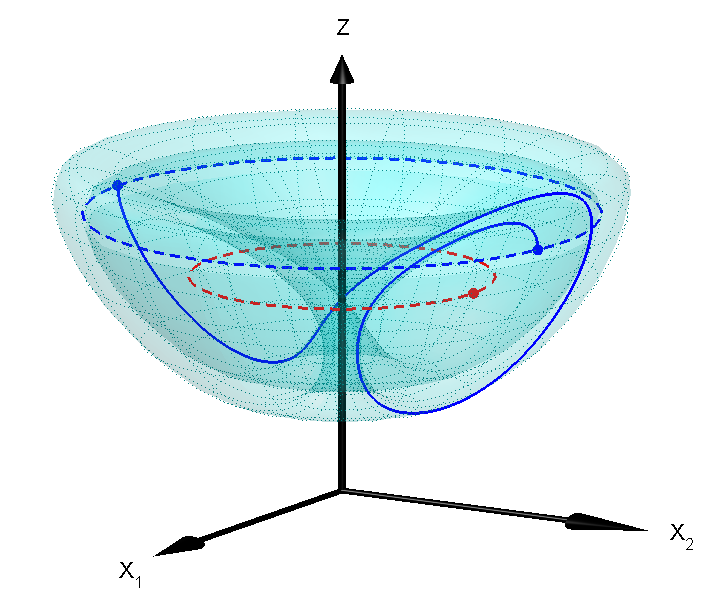
\includegraphics[width=0.35\textwidth,clip=true]{01grouporbit}
\end{center}
  \caption
  [\CLf: $\cycle{01}$ {\rpo} group orbit]{
  \CLf: The \reqv\ $\REQV{}{1}$ is shown by the red dot, and the dashed
  red line is its group orbit / trajectory. One period of the
  $\cycle{01}$ {\rpo} is shown by the solid blue line. The group orbit of
  its (arbitrary) starting point is shown by the dashed blue line: after
  one period the trajectory has returned to the group orbit but with a
  different phase. The group orbit of the $\cycle{01}$ trajectory (dark
  blue) is shown by the cyan surface. Trajectory of the further 15
  repeats of $\cycle{01}$ (faint dotted lines) traces out ergodically the
  torus generated by the$\cycle{01}$  group.
  }
\label{fig:CLf01group1}
\end{figure}


\subsubsection{Symmetry-induced coordinate frames}
\label{s:symmIndCoo}

At least locally, presence of a continuous symmetry suggests two
natural mutually orthogonal basis vectors, the group action tangent and
curvature vectors.

Consider the one-parameter rotation group \SOn{2} acting on a smooth
periodic function $u(\gSpace + 2\pi) = u(\gSpace)$ defined on domain
$\gSpace \in [0,2\pi)$, expanded in the Fourier basis
\refeq{eq:ksexp}.
    \PC{replace this by the original, 2\dmn\  real \SOn{2}  representation}
Parametrize the forward
translation by the continuous parameter $\phi$,
\(
    \LieEl(\phi)\,u(\gSpace) = u(\gSpace-\phi)
\,,
\)
or, in the Fourier basis,
\(
   \LieEl(\phi) \,\ssp = \mathrm{diag}\{ \mathrm{e}^{-\mathrm{i}m\phi} \} \,\ssp
\,.
\)
The tangent to the group orbit at the point $\ssp$ is then given by
the first derivative with respect to the group parameter,
\bea
   {\bf t}(\ssp) &=&
   \lim_{\gSpace\to 0}
   \left(\LieEl(\gSpace)\,\ssp - \ssp\right)/\gSpace
   = \mathrm{diag}\{ -\mathrm{i}m \} \, \ssp = \Lg \ssp,
\label{eq:tang}
\eea
where $\normVec$ is a unit vector normal to the tangent. The pair of unit vectors
    \PC{2011-10-28
    ``As $\Norm{\LieEl(\gSpace)\slicep}$ is a constant, for the group tangent
    vector $\Lg_\gSpace \slicep$ evaluated at $\slicep$ \refeq{eq:tang}
    %GroupTangField} is normal to $\slicep$, and the term
    $\braket{\slicep}{\Lg_\theta\,\slicep}$ vanishes ($\Lg_{\theta}$ is
    antisymmetric).''
The state vector $\ssp$ is not normal to \normVec(\ssp), as $\braket{\ssp
\Lg^2}{\ssp} = - \Norm{\groupTan(\ssp)}^2 \neq 0$, but can one use it to
produce from $\ssp$ the 3. local eigenbasis unit vector? Have not thought
that through. If we do that here, need to rewrite text leading to
\refeq{PCsectQ0}.
    }
\beq
\{{\be_n},{\be_{n+1}}\} =
\{\groupTan(\ssp)/\Norm{\groupTan(\ssp)},\normVec(\ssp)\}
\ee{FrenetFrame}
forms a local orthogonal Frenet-Serret frame at $\ssp$, and can be useful
in constructing the \statesp\ basis vector set \refeq{intrSspTraj}.

\begin{figure}
  \centering
(a)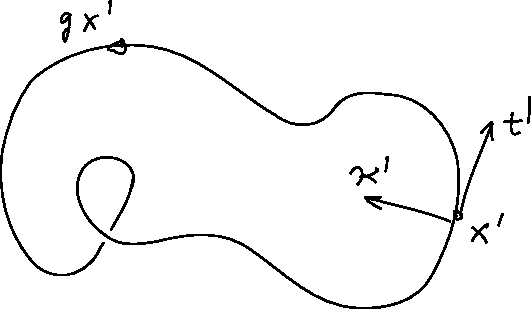
\includegraphics[width=0.20\textwidth]{A29FSframe}
(b)%\includegraphics[width=0.45\textwidth]{2840GOt135th0}
  \caption{\label{fig:2840GOt135th0}
    %\label{fig:M1groupOrb}
Projections of group orbits of two states $\ssp$ (in $\approx
100,000$-dimensional {\statesp}) onto a stationary Frenet-Serret frame
given by unit vectors in the directions
$\{\groupTan_z(\ssp'),\groupTan_\theta(\ssp'),\normVec_z(\ssp')\}$ (see
\refeq{FrenetFrame}). The group orbit is generated by
$\LieEl(0,\shift)\,\ssp$, i.e. by axial shifts, and plotted relative to the
point $\ssp'$.
In  (b) $\ssp$ is a strongly nonlinear chaotic state.
Group orbits are only topologically circles, and inflections are possible
when $\ssp$ is not so close to $\ssp'$.
%{APW 111027 For N2_UB, only see mild distortions;
% see fig 15(b) of dailyBlog}
  }
\end{figure}

For a time-dependent group parameter
$\gSpace$, the phase speed $\dot{\gSpace}$ along the group tangent
evaluated at the \statesp\ point $\ssp$ (the `Cartan derivative') is
given by
\beq
\LieEl^{-1}\dot{\LieEl} \,\ssp % =e^{-\gSpace \cdot \Lg} \,
     =\mathrm{e}^{-\gSpace \Lg} \,
\left(\frac{\mathrm{d} ~~}{\mathrm{d} \, \zeit} \, % e^{\gSpace \cdot \Lg}\ssp
                             \mathrm{e}^{\gSpace \Lg}\right)\ssp
    =\dot{\gSpace} \, \groupTan(\ssp)
%    =\dot{\gSpace}\cdot \groupTan(\ssp)
\,.
\ee{CartanDer}



\subsubsection{Ring of Fire}

%%%%%%%%%%%%%%%%%%%%%%%%%%%%%%%%%%%%%%%%%%%%%%%%%%%%%%%%%%%%%%%%%%%%%
\begin{figure}
(a) 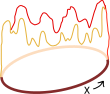
\includegraphics[width=0.145\textwidth]{A27RoFire}
(b) 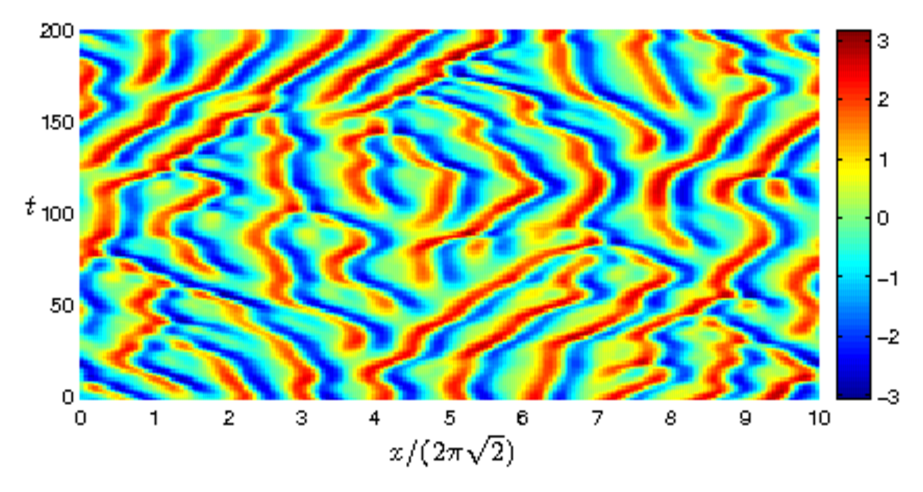
\includegraphics[width=0.255\textwidth]{ks_largeL_cbar_200}
  \caption{
The Ring of Fire, visualized as
    (a)
a Bunsen burner flame flutter, with $u=u(x,t)$ the velocity of the
flame front at position $x$ and time $t$;
    (b)
a spatiotemporal plot (from \wwwcb{}). The symmetry of the system is
$\On{2}$; a rotation of a solution is also a solution.
  }
\label{fig:A27RoFir}
\end{figure}
%%%%%%%%%%%%%%%%%%%%%%%%%%%%%%%%%%%%%%%%%%%%%%%%%%%%%%%%%%%%%%%%%%%%%

Bunsen burner, invented by G\"ottingen chemistry prodigy Robert Bunsen in
1855, entered popular culture in  in 1963 as Johnny Cash
\etal\rf{CaCaKi63} ``\HREF{http://www.youtube.com/watch?v=mIBTg7q9oNc}
{Ring of Fire}'' (\reffig{fig:A27RoFir}), and its flame front
instabilities were modeled in 1976 by Kuramoto\rf{ku} and
Sivashinsky\rf{siv} by one of the simplest nonlinear PDEs that exhibit
spatiotemporally chaotic behavior. The time evolution of the  flame front
velocity $u=u(x,t)$ on a periodic domain $u(x,t) = u(x+L,t)$ is given by
\beq
  u_t = F(u) = -u\,u_x-u_{xx}-u_{xxxx}
    \,.
\ee{ks}
Spatial periodicity $u(x,t)=u(x+L,t)$
makes it convenient to work in the Fourier space,
\beq
  u(x,t)=\sum_{k=-\infty}^{+\infty} a_k (t)\, e^{ i k x /\tildeL }
\,,
\ee{eq:ksexp}
with the $1$-dimensional PDE \refeq{ks}
replaced by an infinite set of
ODEs for the complex Fourier coefficients $a_k(t)$:
\beq
\dot{a}_k= \pVeloc_k(a)
     = ( q_k^2 - q_k^4 )\, a_k
    - i \frac{q_k}{2} \sum_{m=-\infty}^{+\infty} a_m a_{k-m}
\,,
\ee{expan}
where $q_k = 2\pi k/L$.


\subsection{Symmetries of pipe flow}
\label{s:SymmPipe}
% former siminos/atlas/symm.tex



Let $\LieEl(\phi,\shift)$ be the shift operator such that $\LieEl(\phi,0)$
denotes an azimuthal rotation by $\phi$ about the pipe axis,
and $\LieEl(0,\shift)$ denotes the stream-wise translation by
$\shift$; let $\sigma$ denote reflection about the $\theta=0$ azimuthal
angle:
\bea
\LieEl(\phi,\shift) \, [u,v,w,p](r,\theta,z)
        & = & [u,v,w,p](r,\theta-\phi,z-\shift)
			  \continue
\sigma \, [u,v,w,p](r,\theta,z) \;\; & = & [u,-v,w,p](r,-\theta,z)
\label{pipeSymms}
\eea
%
The \NSe\ for pipe flow are equivariant under these transformations. The
symmetry group of stream-wise periodic pipe flow is thus $\Group =
\On{2}_\theta \times \SOn{2}_z = \Dn{1} \ltimes \SOn{2}_{\theta} \times
\SOn{2}_z$, where $\Dn{1} = \{ e,\, \sigma \}$ denotes azimuthal
reflection, $\ltimes$ stands for a semi-direct product (in general,
reflections and rotations do not commute), and the subscripts $z,\theta$
indicate stream-wise translation and azimuthal rotation respectively.



\begin{figure}
  \centering
(a)%\includegraphics[width=0.45\textwidth]{2839GOLB}
(b)%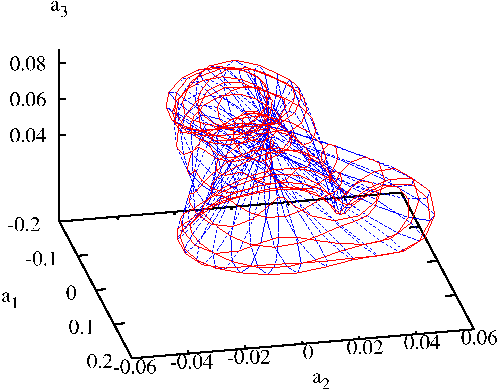
\includegraphics[width=0.45\textwidth]{2840GOt135M1}
  \caption{\label{fig:2830GO6}
    %\label{fig:M1groupOrb}
As \reffig{fig:2840GOt135th0}, but with the
full 2\dmn\ $\SOn{2}_{\theta} \times \SOn{2}_z$ group orbits traced out
by shifts in both $z$ and $\theta$. Loops in solid red correspond to
shifts in $z$, dashed blue loops to shifts in $\theta$.
%(a) \Reqv\ N2\_LB, (b) \Reqv\ N2\_UB.
  }
\end{figure}


In the literature
(see, \eg\ \cite{Recke2010}) such \SOn{2} is often referred to as the
circle group $S^1$, also denoted `one-torus' $T^1$.

\section{How to slice}
\label{s:algorithm}

Our guiding principle is to chose a \slice\ such that the distance
between a `{\template}' state {\slicep} and nearby group orbits is
\emph{minimized}, \ie, identify the point $\sspRed$ on the group orbit
\refeq{sspOrbit} of a nearby state $\ssp$ which is the closest match to
the {\template} point {\slicep}.

\refFig{fig:sliceimage}, new proposal: take points on the good,
    blue \po, run each along the group orbit until $\sspRSing \in S$
    where it intersects the \sliceBord, see \refeq{sspRSing}, and thus plot
    the border of where the local slice ends, once on the left, and once
    on the right of the {\template}. Catch - I have not thought this
    through, not sure that the condition \refeq{sspRSing} can be
    satisfied on every group orbit...

We have seen that in presence of the continuous $\SOn{2}$ symmetry
\reqva\ and \rpo s are 2- and 3-dimensional manifolds of physically
equivalent states. How are we to compare a pair of such states? We shall
do this here by determining the minimal distance between them.

In particular, even though the
simplest solutions (laminar, \etc) often capture important physical
features of a flow, most \eqva\ and short \po s have nontrivial
symmetries and thus are not suited as choices of symmetry-reducing
{\template s}.

%%%%%%%%%%%%%%%%%%%%%%%%%%%%%%%%%%%%%%%%%%%%%%%%%%%%%%%%%%%%%%%%%%%%%
\begin{figure}
   \centering
(b)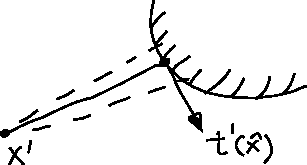
\includegraphics[width=0.20\textwidth]{A28extremum}
   \caption{\label{fig:A28extremum1}
    (b) Extremal condition \refeq{PCsectQ0}, replaced by
    \reffig{fig:A28extremum}
}
\end{figure}
%%%%%%%%%%%%%%%%%%%%%%%%%%%%%%%%%%%%%%%%%%%%%%%%%%%%%%%%%%%%%%%%%%%%%

\subsection{Rotation into the \slice}

As long as the norm is discretization independent, the \slice\ condition
\refeq{PCsectQ0} is independent of the numerical representation $\ssp$ of
the flow $\vec{u}$, be it finite difference, spectral, and so on. The
slice condition is solved for $\shift$ every few time steps using
Newton's method, where a good initial guess for $\shift(\zeit)$ is
obtained from the previous value and $\dot{\shift}(\zeit)$.

To avoid this, a global
atlas has to be pieced together from local \slice\ charts, fixed by
a well-chosen set of
\template s $\slicep{}^{(j)}$.
Shifts $\shift_j(\zeit)$ are tracked for each local \slice\ chart $\pS{}^{(j)}$,
such that the next $\shift_{j+1}(\zeit)$ is selected at intersection with
$\pS{}^{(j+1)}$
to minimize $\Norm{{\ssp}-{\ssp_i}}$.

%\APW{111104 The first sentence requires simplifying!}
As group orbits % of compact Lie groups
are smooth manifolds, have natural linear
representations (under linear action of a symmetry group, \statesp\
decomposes into a sum over irreducible subspaces), and have natural local
coordinate frames (the group tangent, curvature Frenet-Serret frames
\refeq{FrenetFrame}), good \slice s should be easier to construct than
the elusive ``good'' Poincar\'e sections of the time-evolution flows.
Indeed, as a generic \slice\ \refeq{PCsectQ0} is the set of all
group-orbit points closest to a given {\template}, it slices the group
orbits of \emph{all} full \statesp\ points\rf{FrCv11}. However, for a
nonlinear flow, there is no single \slice\ that really does the job: our
\slice\ is locally a hyperplane, expected to be a good description of
solutions similar to a given {\template} in some open neighborhood. The
variational distance condition \refeq{PCsectQ0} is only an extremum
condition, and as the group orbits of highly nonlinear states are highly
contorted (see \reffig{fig:2830GO6}\,{\it b}), they can have many
extrema, and multiple sections by a \slice\ hyperplane. For example, an
\rpo\  torus is always intersected by a \slice\ hyperplane in two or more
sections, see \reffig{fig:sliceimage}.

    \ifdraft\color{blue}
        {\bf 2012-03-15 Predrag} \refFig{fig:sliceimage}, new proposal:
        take points on the good, blue \po, run each along the group orbit
        until $\sspRSing \in S$ where it intersects the \chartBord, see
        \refeq{sspRSing}, and thus plot the border of where the local
        slice ends, once on the left, and once on the right of the
        {\template}. Catch - I have not thought this through, not sure
        that the condition \refeq{sspRSing} can be satisfied on every
        group orbit...
    \color{black}\fi

It should be emphasized that we never need to integrate the reduced
equations \refeq{EqMotMFrame}; numerical simulations are always carried
out in the full \statesp. Slicing is implemented as postprocessing of
numerical or experimental data, by rotating full \statesp\ trajectories
into the \slice, as in \reffig{fig:sliceimage}.

The apparent divergence in {\phaseVel} \refeq{reconstrEq} is a
non-physical artifact of the symmetry reduction by tangent hyperplanes,
but a numerical nuisance nevertheless. Here is how we avoid it.

\subsection{Physical dimension: covariant Lyapunov vectors}

\subsection{Dynamically important solutions and Newton's method}
\label{s:reqva}

The way in which the \mslices\ enables to find initial
guesses for $(\vec{u}(0),\period{},\shift)$, is the main differences
between this study and the previous ones.

Here we take as initial guesses samples of nearly recurrent velocity
fields generated by long-time simulations of turbulent dynamics
\rf{pchaot,CviGib10}. The intent is to find the {\em dynamically most
important} solutions, by sampling the turbulent flow's natural measure.
In practice, sufficiently good full \statesp\ initial guesses for
$(\vec{u}(0),\period{},\shift)$ would be almost impossible to find.
Checking correlations between $\vec{u}(\zeit)$ and
$\LieEl(0,\shift)\,\vec{u}(\zeit-\period{})$ for each $\period{}$, and
more problematically, for all possible shifts $(\phi,\shift)$, is an
unrealistic task. The \mslices, however, enables us determine close
recurrences  from the symmetry-reduced time series, and locates the
dynamically most important solutions, \ie, those trajectories that are
most likely to be observed in a long-time turbulent simulation. The \rpo
s are reduced to \po s, whose unstable manifolds are much easier to track
in the \reducedsp. The \rpo\ shift $\shift$ is given by the
reconstruction equation, \refeq{reconstrEq}, or, in practice, by phase
shift $\shift(\period{})-\shift(0)$ accumulated by the intermediate
Newton steps that keep the orbit within the slice.

Without symmetry reduction, the detection of the nearest recurrence of a
state near a previous state, earlier on the the same trajectory, would
require the calculating the minimum over all possible shifts. Within the
symmetry-\reducedsp\ the determination of recurrences is simple, as the
slices are constructed by requiring that the slice points are the minimum
distance points between the group orbits of the two states.

These are not the `modes' of the fluid; {they
do not provide a decomposition of the flow into a sum of components at
different wavelengths, or a basis for low-dimensional
modeling.} Each such solution spans the whole range of physical scales of
the turbulent fluid, from the outer wall-to-wall scale, down to the
viscous dissipation scale. Numerical computations require sufficient
resolution to cover all of these scales, so no {global} dimension
reduction is likely.

        {\bf PC 2011-10-18} Note also that the rotation of a fluid flow
        into a \slice\ {\em is not} an average over the 3D pipe azimuthal
        angle, it is the full snapshot of the flow embedded in the
        $\infty$-dimensional \statesp.

the Cartan derivative \refeq{CartanDer}.

As a generic \slice\ \refeq{PCsectQ0} is the set of all group-orbit
points closest to a given {\template}, it slices the group orbits of
\emph{all} full \statesp\ points\rf{FrCv11}.

A single
\slice\ hyperplane cannot do the job well. As the {\nws} of the dynamics is a
highly contorted, nonlinear curved manifold embedded in a
high-dimensional \statesp, any such linearization is good only locally: a
single {\template} cannot be a good match  globally. The variational
distance condition \refeq{PCsectQ0} is an extremum condition, and as the
group orbits of highly nonlinear states are highly contorted (see
\reffig{fig:2830GO6}\,{\it b}), the distance function can have many
extrema, and multiple sections by a \slice\ hyperplane. For example, a
\rpo\ sweeps out a torus, and is always intersected by a \slice\
hyperplane in two or more \po\ sections, once at the orbit's closest
passage to the template, and another time at the most distant passage,
also satisfying the slice condition  \refeq{PCsectQ0} (see
\reffig{fig:sliceimage}\,{\it a}).

The role of invariant solutions is
to partition the $\infty$-dimensional \statesp\ into a finite set of
neighborhoods visited by a typical long-time turbulent fluid state.

Ignore it at
your own peril; the invariant solutions found by restricting
searches to the discrete-symmetry invariant subspaces have little if
anything to do with the full \statesp\ explored by turbulence, not more
than the \eqv\ points of the Lorenz equation have to do with its strange
attractor.
